\documentclass[11pt]{article}
\usepackage[utf8]{inputenc}
\usepackage[margin=1in]{geometry}

\usepackage{algorithm}
\usepackage[noend]{algpseudocode}
\algnewcommand\Or{\textbf{ or }}
\algnewcommand\Init{\textbf{initialize }}
\MakeRobust{\Call}

\usepackage{natbib}
\usepackage{graphicx}
\usepackage{epigraph}
\usepackage{float}
\usepackage{tikz}
\usepackage{float}
\usepackage{algorithm}
\usepackage{algpseudocode}
\algrenewcommand{\algorithmicreturn}{\State \textbf{return}}
\usetikzlibrary{graphdrawing}
\usetikzlibrary{graphs}
\usegdlibrary{trees}

\title{Treaps}
\author{Justin Zhang}
\date{16 February 2018}

\begin{document}

\maketitle


\section{Introduction}

Balanced binary search trees (BBSTs) can be very useful in data structure problems due to their flexibility. They can be used to replace a number of data structures we've covered up until now (e.g. segment trees and BITs). In general, they are used to represent an ordered set (store and check if an element exists in the set) in $O(\log n)$ time. However, by augmenting the nodes, we can use BBSTs for a much larger variety of problems, such as range min/max and sum queries.

That being said, BBSTs are often very tedious to implement. Red-Black trees depend heavily on casework. AVL trees and splay trees have a confusing rebalancing routine, and are harder to implement.

Treaps are randomized BBSTs that are very easy to implement. However, their trade-off is that they do not guarantee logarithmic time, and can be linear time in the worst case (due to their random nature). However, they are almost always logarithmic, and can be treated as such for competitive programming.

\section{Treap implementation}

The key idea behind a treap is to augment the nodes in a binary search tree (BST) each with a unique, randomly chosen number $R$. Then, we ensure that our keys $K$ follow the standard BST ordering (left subtree smaller and right subtree greater) and that the randomly chosen number $R$ follows the max-heap property. In this way, we combine a BST and a heap (hence ``treap").


    \begin{figure}[H]
        \centerline{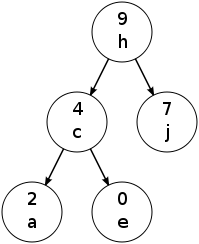
\includegraphics[scale=0.5]{treap.png}}
        \caption{A treap, where the numbers are our randomly chosen numbers $R$ and the letters are our keys $K$.}
        \label{fig:treap}
    \end{figure}
    
Note that there is always at least one configuration of the tree that satisfies both the BST and max-heap property.

To see this, consider the node with maximal $R$. This is the root. Then we can divide our nodes into those with a lower $K$ and those with a greater $K$, and recursively form treaps at the left and right subchildren. Clearly, then, there must always exist a valid treap configuration.



\subsection{Rotations}
    \begin{figure}[h!]
\centering
\begin{tikzpicture}[>=stealth, every node/.style={circle, draw, minimum size=.75cm}]
\graph [tree layout, grow=down, fresh nodes, level distance=0.5in, sibling distance=0.75in]
    {
        d -> {
          b -> { A, C },
          E
        },
        b -> {
          A,
          d -> { C, E }
        },
    };
\end{tikzpicture}
\caption{Tree rotations.}
\label{fig:rotation}
\end{figure}

Like in AVL trees, we use tree rotations as a way to ensure that the BST ordering is kept while modifying the tree structure (more on why we'd want that later). A \textit{right} tree rotation would go from the left tree to the right, and a \textit{left} tree rotation would go from the right to the left.

A, C, and E represent subtrees of arbitrary size, and b and d are specific keys, such that $\verb|all nodes in A| < b < \verb|all nodes in C| < d < \verb|all nodes in E|$.

\subsection{Treap Search}
    We do a standard binary search tree search here. Starting at the root, we compare the key to our search value. If the key is greater, we move left and recurse. If it's less than, we move right and recurse. Else we've found our value, and we're finished.
    
    This is clearly $O(H)$ time, where $H$ is the height of our tree.
    
\subsection{Treap Insert}
    To insert, we first perform a standard binary search tree insert. That is, we follow the tree as if we were doing a search. Then, we add a new node with our value and a randomly generated number $R$ as a leaf.
    
    We must now ensure the heap property is satisfied. Note that we cannot do the typical ``bubble up" heap algorithm, since this could violate the BST ordering. Thus, we use rotations instead.
    
    If our current node's $R$ is larger than its parent's $R$:
    
    \begin{enumerate}
        \item If we're a left subchild, perform a right tree rotation
        \item If we're a right subchild, perform a left tree rotation
    \end{enumerate}
    
    We can then recurse upward. Since rotations are constant time, this is $O(H)$ time, where $H$ is the height of our tree.
    
\subsection{Treap Delete}
    We have two cases for delete. If the node in question is a leaf, we can just remove it. Otherwise, we must bring it to the bottom of the tree so that it's a leaf, then remove it.
    
    To bring it down, we set the $R$ value to $-\infty$. Then we do tree rotations to preserve the max-heap property:
    
    \begin{enumerate}
        \item If the left subchild's $R$ is less than our right subchild's $R$, we rotate left
        \item Otherwise we rotate right
    \end{enumerate}
    
    We can then recurse downward. This is similarly $O(H)$ time, where $H$ is the height of our tree.
    
\section{Treap Height}
    Why is a treap's height (usually) logarithmic?
    
    The math proving it isn't \textit{that} complicated, but it involves some infinite sums, and is out of the scope of this lecture. But intuitively...
    
    Consider this: given a treap, say we're at the root. The probability of a subtree's size being less than $\frac{3}{4}n$ is $\frac{1}{2}$. Thus, every time we go down a level, we expect that we will have a geometric decrease (of a factor of $\frac{3}{4}$). This implies a logarithmic complexity.
    
    Mathematically, a treap's height $H$ will be approximately $2 \ln n$. More precisely, we know that it's bounded as such: $$ P(H > 2\,c\,\ln n) < n (n/e)^{-c\,\ln(c/e)}$$
    
    Where $c$ is any arbitrary positive number.
    
    This implies, with $n = 10^5$, if we choose $c = 4.5$,
    $$ P(H \geq 104) < 4.4 * 10^{-6} $$
    
    In other words, for $n = 10^5$, the probability that $H > 6.24 \log n$ is less than $4.4 * 10^{-6}$.
    

\section{Problems}

\begin{enumerate}
    \item How can we augment the BBST to effectively function as a min, max, and sum segment tree? In what cases can we do it the other way around?
    
    \item SPOJ KPMATRIX: Given a $N$x$M$ matrix of integers ($1 \leq N,M \leq 250)$, and two integers $A$ and $B$ ($-10^9 \leq A, B \leq 10^9$), find the number of submatrices with sum between $A$ and $B$.
    
    \item SPOJ GSS6: Given an integer array of length $N$, apply $Q$ operations which can be any of inserting an element, deleting an element, and finding the maximal contiguous non-empty sum in a given interval ($1 \leq N, Q \leq 10^5$). All values in the array, as well as insertions, are between $-10^4$ and $10^4$.
\end{enumerate}


\end{document}
